%% document class
\documentclass[10pt]{beamer}
%%theme
\usetheme[hideothersubsections,width=2cm]{Berkeley}
%% page settings
\usepackage{xcolor}
\usenavigationsymbolstemplate{}
\usefonttheme{serif}

%% packages
\usepackage{tikz}
\usepackage{geometry}
\usepackage{mathptmx}
\usepackage[scaled=0.9]{helvet}
\usepackage{courier}

%%color settings
%%%%% Color Schema

\definecolor{blue_dark}{RGB}{38,50,56}
\definecolor{blue}{RGB}{33,150,243}
\definecolor{blue_light}{RGB}{79,195,247}
\definecolor{grey_dark}{RGB}{38,50,56}
\definecolor{grey}{RGB}{33,150,243}
\definecolor{grey_light}{RGB}{33,150,243}

%% theme settings
\setbeamercolor*{palette primary}{fg=grey_dark,bg=blue_light} % upper part
\setbeamercolor*{palette secondary}{fg=grey_dark,bg=blue_light} % left part (background)
\setbeamercolor*{sidebar left}{fg=blue_light,bg=grey_dark} % left part with links
\setbeamercolor*{palette sidebar primary}{fg=blue_light}
\setbeamercolor*{palette sidebar secondary}{fg=blue_light}
\setbeamerfont{section in sidebar}{size=\scriptsize}

%% new commands
%\input{settings/macros}
\addtobeamertemplate{frametitle}{\vskip+0.6ex}{}
\makeatletter
\beamer@headheight=2\baselineskip
\makeatother

\begin{document}

\author[Group 9]{Suvojit Manna\\Pronab Mukherjee\\Barun Gupta\\Somnath Rakshit\\}
\title[Machine Learning]{Introduction to Machine Learning using \LaTeX}
%\logo{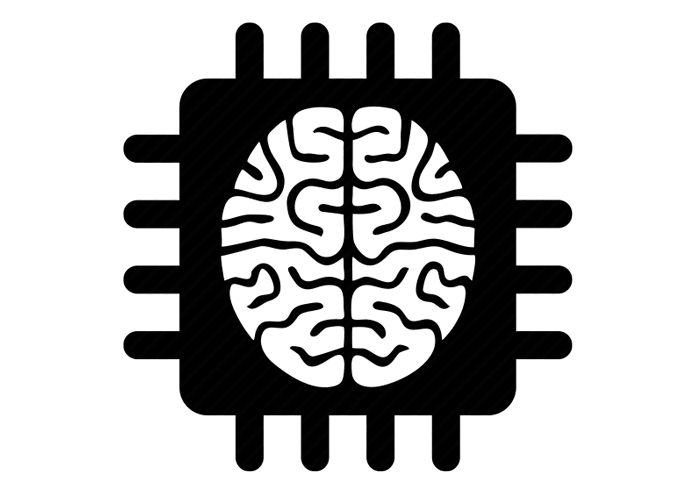
\includegraphics[width=4mm]{images/icon}}
\institute[JGEC]{Jalpaiguri Govt Engineering College}
%\date{City, date}


%% Title Page
\begingroup
\setbeamercolor{background canvas}{bg=blue_dark}
\begin{frame}[plain,t]
	\hspace*{-22 mm}
	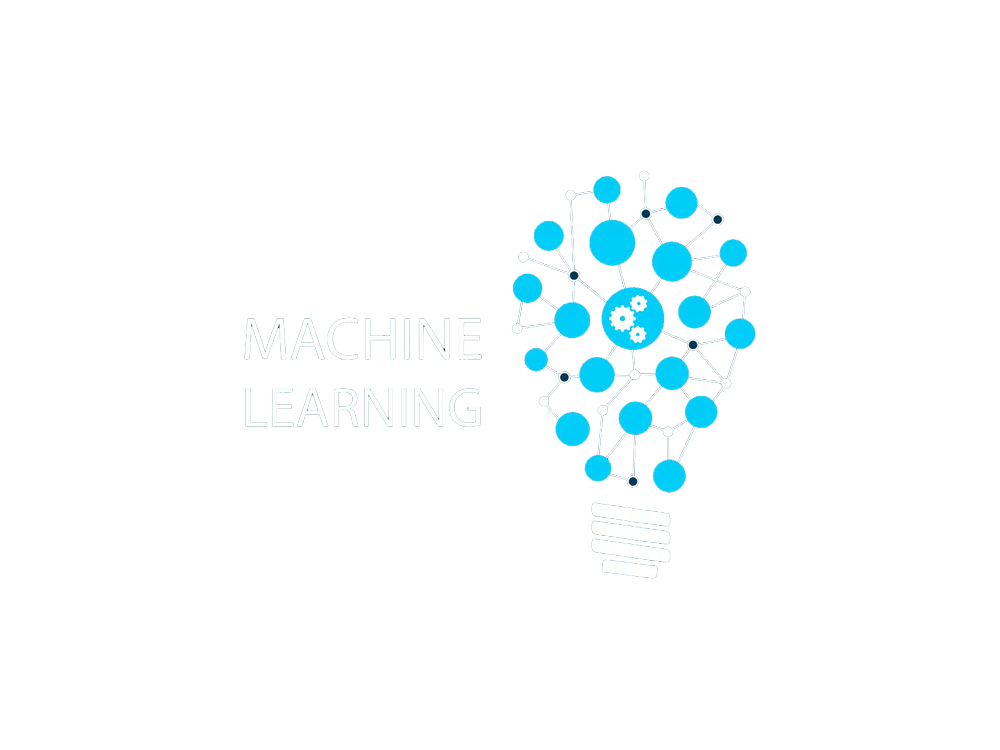
\includegraphics[width=\paperwidth,height=\paperheight]{images/ml_bg}
\end{frame}
\endgroup

%% A Team Page
\begingroup
	\usebackgroundtemplate{%
		\tikz\node[opacity=0.3] {
\includegraphics[height=\paperheight,width=\paperwidth]{images/bg-vec}}
		;}
	\begin{frame}[c]{The A Team}
		\begin{center}
			\Huge{Presented By:\\}
			\large{~\\Suvojit Manna\\Pronab Mukherjee\\Barun Gupta\\Somnath Rakshit\\}
		\end{center}
	\end{frame}
	%% contents
	\begin{frame}{Contents in Brief}
		%\tableofcontents
		\tableofcontents[hideallsubsections]
	\end{frame}
\endgroup
	%% Big Font Page: Lets get started
\begingroup
	\setbeamercolor{background canvas}{bg=blue_dark}
	\setbeamercolor{normal text}{fg=blue_light}
	\begin{frame}[plain,c]
		\hspace*{10 mm}
		\vspace*{-18 mm}
		\textcolor{blue_light}{\Huge{Let's Get Started}}
	\end{frame}
\endgroup


\begingroup
	\usebackgroundtemplate{%
		\tikz\node[opacity=0.3] {
\includegraphics[height=\paperheight,width=\paperwidth]{images/bg-vec}}
		;}
	
	\section{Introduction}
		\begin{frame}{Machine Learning | What ?}
			\begin{center}
				\large{Field of study that gives computers the ability to learn without being explicitly programmed.}\\
				\bigskip
				\small{Instead of writing code, you feed data to the generic algorithm and it builds its own logic based on the data.}
				%TODO : Insert Image
			\end{center}
		\end{frame}
		\subsection{Case Studies}
			\begin{frame}{Case Studies | Machine Learning}
			\end{frame}
		\subsection{Formal Defintion}
			\begin{frame}{Machine Learning | Formal Definiton}
				\begin{center}
					\small{The field of machine learning is concerned with the question of how to construct computer programs that automatically improve with experience.}\\
					\bigskip
					\large{A computer program is said to learn from experience E with respect to some class of tasks T and performance measure P, if its performance at tasks in T, as measured by P, improves with experience E.}\\
					\bigskip
					\text{Evolved from :}
				\end{center}
			\end{frame}
		\subsection{Benefits}
			\begin{frame}{Benefits | Machine Learning}
			\end{frame}
		\subsection{Applications}
			\begin{frame}{Applications | Machine Learning}
			\end{frame}
	
	\section{Regression}
		\begin{frame}{Introduction | Regression}
		\end{frame}
		\subsection{Usages}
			\begin{frame}{Usages | Regression}
			\end{frame}
		\subsection{Benefits}
			\begin{frame}{Benefits | Regression}
			\end{frame}
		\subsection{Example Cases}
			\begin{frame}{Example Cases | Regression}
			\end{frame}
	
	\section{Classifications}
		\begin{frame}{Introduction | Classifications}
		\end{frame}
		\subsection{Usages}
			\begin{frame}{Usages | Classifications}
			\end{frame}
		\subsection{Example Cases}
			\begin{frame}{Example Cases | Classifications}
			\end{frame}
	
	
	\section{Deep Learning}
		\begin{frame}{Introduction | Deep Learning}
		\end{frame}
		\subsection{Neural Networks}
			\begin{frame}{Neural Networks | Deep Learning}
			\end{frame}
		\subsection{Meaning}
			\begin{frame}{Meaning | Deep Learning}
			\end{frame}
		\subsection{Usages}
			\begin{frame}{Usages | Deep Learning}
			\end{frame}
		\subsection{Advantages}
			\begin{frame}{Advantages | Deep Learning}
			\end{frame}
	
	
	
	\section{Conclusion}
		\begin{frame}{The pain is almost over}
		\end{frame}
		\begin{frame}{Bibliography}
			\twocolumn
			\begin{itemize}
				\item \scriptsize{Phil Simon (March 18, 2013). Too Big to Ignore: The Business Case for Big Data. Wiley. p. 89. ISBN 978-1-118
					-63817-0.}
				\item \scriptsize{Mitchell, T. (1997). Machine Learning, McGraw Hill. ISBN 0-07-042807-7}
			\end{itemize}
			\onecolumn
		\end{frame}
\endgroup

\begingroup
	\setbeamercolor{background canvas}{bg=blue_dark}
	\setbeamercolor{normal text}{fg=blue_light}
	\begin{frame}[plain,c]
		\hspace*{6 mm}
		\vspace*{-18 mm}
		\textcolor{blue_light}{\Large{Now that was very interesting!}}
	\end{frame}
	\begin{frame}[plain,c]
		\hspace*{27 mm}
		\vspace*{-20 mm}
		\textcolor{blue_light}{\Large{The End}}
	\end{frame}
\endgroup

\end{document}


